\chapter{Results\label{chap:Results}}
This chapter describes the results of the two experiments conducted for this thesis.  Statistical models and post\-/hoc acoustic analyses that help to clarify and explain the results are also presented.

\section{Experiment 1}
Experiment~1 tests the role of prosody in intelligibility, by comparing mean sentence scores for unmodified talkers against resynthesized stimuli with prosodic replacement.  A quartile analysis indicated a significant improvement in performance between the first and last quartiles (\textit{t}=−3.016 on 709.3 degrees of freedom, \textit{p}<0.01; see Figure~\ref{fig:ExpOneQuartile}).  The magnitude of the difference between the first and fourth quartiles is approximately 0.4 keywords.

\begin{figure}[bt]
	\begin{centering}
	\includegraphics{figures/results/ExpOneQuartileBarplot.eps}
	\caption[Mean sentence scores by quartile for Experiment~1]{Mean sentence scores by quartile for Experiment~1.  Error bars are ±1 standard error.\label{fig:ExpOneQuartile}}
	\end{centering}
\end{figure}

The mean sentence score for each talker across listeners is shown in Figure~\ref{fig:ExpOneBarplot}.  Darker bars indicate unmodified stimuli, while light bars represent resynthesized stimuli.  It is noteworthy that not all resynthesized stimuli have lower mean scores compared to their unmodified counterparts, suggesting that distortion due to the resynthesis process was relatively minimal.  This is likely due to several factors; one is probably the painstaking hand\-/correction of the pulse marks during stimulus preparation, which ensured consistent phase of the \fo{} epochs throughout voiced spans of speech.  Another possible explanation for the low levels of distortion is the choice to maintain each talker’s natural mean pitch on each sentence, and map only the {\emph shape} of the pitch contour of the prosodic donor during resynthesis.  

With regard to Research Question~1 — \emph{how does prosody relate to intelligibility?} — a complex picture emerges.  Talker~\ac{b} suffers dramatically when his prosody is replaced, whereas Talker~\ac{c} is unchanged or slightly improved, and Talker~\ac{a} is unchanged or slightly worsened.  One possible explanation for these results is to postulate that Talker~\ac{a}, despite being highly intelligible, does not have especially good prosody, evidenced in particular by the fact that scores for Talker~\ac{ca} are lower than the scores for Talker~\ac{cb}.  On the same grounds, and on the additional observation that scores for Talker~\ac{ab} are greater than for Talker~\ac{ac}, we might conclude that Talker~\ac{b} has more intelligible prosody than the other two talkers, and his middling base intelligibility scores are due to segmental factors.

\begin{figure}[bt]
	\begin{centering}
	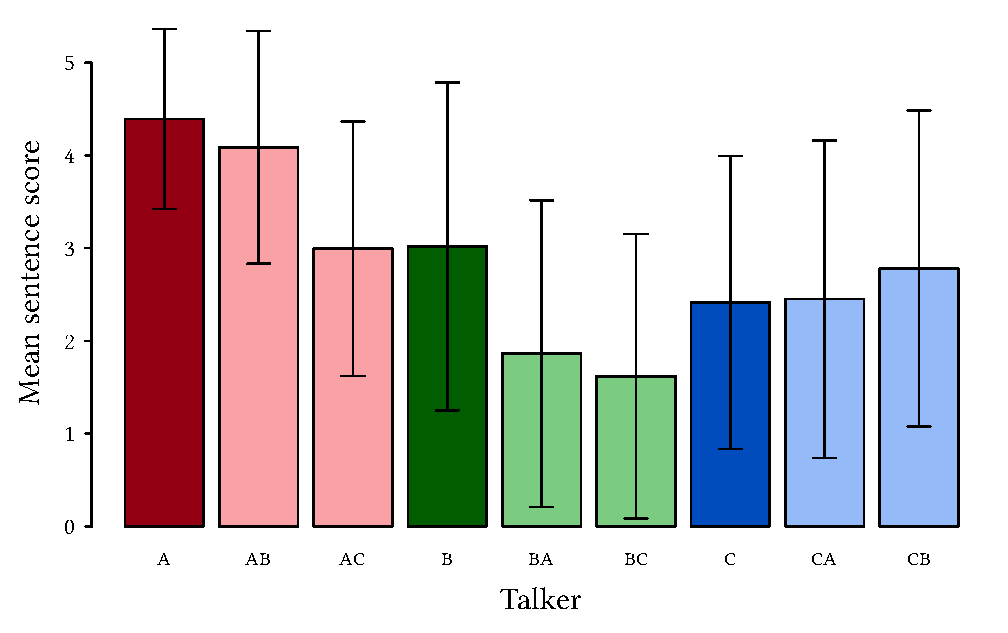
\includegraphics{figures/results/ExpOneBarplot.eps}
	\caption[Barplot of mean sentence scores for Experiment~1]{Barplot of mean sentence scores for Experiment~1.  Error bars are ±1 standard error; lighter colors indicate resynthesized talkers, with the second letter indicating the prosodic donor (see Section~\ref{sec:ExpDesign} for full explanation of talker codes).  Similar hues indicate shared segmental donors.\label{fig:ExpOneBarplot}}
	\end{centering}
\end{figure}

With regard to the question of whether low\-/intelligibility talkers can be made more intelligible through prosody alone, it would appear that the answer is “yes”: Talker~\ac{cb} appears to have higher scores than Talker~\ac{c}, despite the likelihood that Talker~\ac{cb}’s recordings suffer some amount of distortion from the resynthesis process, however small.  In other words, any degradation due to resynthesis seems to have been more than overcome by the benefit of having Talker~\ac{b}’s prosody mapped onto Talker~\ac{c}’s signal.  However, it is noteworthy that the greatest improvement to Talker~\ac{c}’s intelligibility does not come from Talker~\ac{a}’s prosody, even though Talker~\ac{a} has the highest overall intelligibility.  This suggests that high\-/intelligibility talkers do not necessarily use prosody that enhances their intelligibility.

\subsection{Experiment~1 statistical model}
To further probe these results, the scores were submitted to a mixed\-/effects linear regression model, shown here:%in Equation~\ref{eq:ExpOneMM}:

\noindent{\small\inlinecode lmer(sentScore\textasciitilde resynth+segDonor+proDonor+trial+(1|listener)+(1|sentence))}
%\begin{equation}\label{eq:ExpOneMM}
%	\text{{\small \inlinecode lmer(sentScore\textasciitilde resynth+segDonor+proDonor+(1|listener)+(1|sentence), data=allData)}}
%\end{equation}

In this model, the dependent variable {\inlinecode sentScore} is the number of keywords correct (0–5), and is being predicted by several independent variables: {\inlinecode resynth} is a Boolean variable that is true for Talkers~\ac{ab}, \ac{ac}, \ac{ba}, \ac{bc}, \ac{ca} and~\ac{cb}, and {\inlinecode segDonor} and {\inlinecode proDonor} are three\-/level factors indicating the talker in the target signal and the talker from whom the prosodic information was drawn, respectively.  For the unmodified original recordings, {\inlinecode segDonor} and {\inlinecode proDonor} are defined as the talker himself, even though those recordings were not resynthesized.  The effect of task familiarization seen in Figure~\ref{fig:ExpOneQuartile} is accounted for by the fixed\-/effect predictor {\inlinecode trial} (a numeric value ranging from 1–90).  Two random\-/effects predictors ({\inlinecode 1|listener} and {\inlinecode 1|sentence}) are also included to model variability in listener performance and sentence difficulty, respectively. 

%A summary of the model shown in Equation~\ref{eq:ExpOneMM} 
A summary of fixed\-/effects predictors for this model is given in Table~\ref{tab:ExpOneFixedEff}.  All fixed\-/effects predictors were significantly different from zero, and there was no evidence of correlation of fixed effects (correlation coefficients all less than 0.1; not shown).  The baseline condition is Talker~\ac{a}, with a value at the intercept of about 4.1 words correct.  The coefficients reveal similar patterns to those seen in Figure~\ref{fig:ExpOneBarplot}: firstly, the model supports the interpretation that Talker~\ac{b} has the most intelligible prosody.  Having the prosody of Talker~\ac{b} represents a net gain of 0.3 words correct over the prosody of Talker~\ac{a}, whereas having the prosody of Talker~\ac{c} represents a net loss of more than 0.6 words correct compared to Talker~\ac{a}.  The model also supports the idea that Talker~\ac{a}’s intelligibility stems in large part from non\=/prosodic factors, given that the other levels of {\inlinecode segDonor} both have strongly negative coefficients.  The estimated degradation due to resynthesis is about −0.7 keywords correct.  Because trial was a continuous variable ranging from 1–90, the coefficient for the effect of trial is misleadingly small; the predicted difference between the first and the last trial due to listener adaptation to the task is actually 90×0.005549, or 0.5 keywords.

\begin{table}[tbp]
	\caption[Experiment~1 statistical model: Fixed effects]{Summary of fixed effect predictors in the statistical model of Experiment~1.  \textit{s}: standard error of the coefficient estimate; \textit{t}: \textit{t}\=/value of coefficient estimate; \textit{p}: \textit{p}\=/value of coefficient estimate (calculated via \ac{mcmc}).\label{tab:ExpOneFixedEff}}
	\centering
	\begin{tabu} spread 1em {Xrcrc}
		\toprule
		\multicolumn{5}{l}{Summary of fixed effects (N=1440; log-likelihood=−2551)}\\
		\rowfont\bfseries
		\multicolumn{1}{l}{Predictor} & \multicolumn{1}{c}{Coefficient} & \textit{s} & \multicolumn{1}{c}{\itshape t} & \textit{p}\\
		\midrule
		Intercept         &  4.132 & (0.145) &  28.44 & <10⁻¹⁶\\
		resynth = TRUE    & −0.662 & (0.077) &  −8.63 & <10⁻¹⁶\\
		segDonor = \ac{b} & −1.673 & (0.089) & −18.86 & <10⁻¹⁶\\
		segDonor = \ac{c} & −1.278 & (0.089) & −14.31 & <10⁻¹⁶\\
		proDonor = \ac{b} &  0.307 & (0.088) &   3.48 & <10⁻³\\
		proDonor = \ac{c} & −0.646 & (0.088) &  −7.36 & <10⁻¹²\\
		trial             &  0.006 & (0.001) &   4.02 & <10⁻⁴\\
		\bottomrule
	\end{tabu}
\end{table}

A summary of the random effects in the model for Experiment~1 are shown in Table~\ref{tab:ExpOneRandomEff}.  The results here are not unexpected: the variance in intercepts due to particular listeners doing systematically better or worse on the task is only about 2\% of the total residual variance.  This suggests that, by and large, all listeners were performing equally well on the task.  The variance in intercepts due to varying difficulty of particular sentences is somewhat larger (about 22\% of the total residual variance, or a standard deviation of 0.7 keywords correct),\footnotemark{} suggesting that there was indeed some value in modeling the sentences as varying in their difficulty (cf. the discussion of scoring in Section~\ref{sec:Scoring}).
\footnotetext{The \ac{mcmc} estimate for variability due to listener is in close agreement with the fitted model.  The \ac{mcmc} estimate for variability due to sentence is slightly smaller than the value in the fitted model, at 16\% of the total variance (\vs\ 22\%), with a standard deviation for sentence of about 0.6 keywords (\vs\ 0.7).}

\begin{table}[tbp]
	\caption[Experiment~1 statistical model: Random effects]{Summary of random effects in the statistical model of Experiment~1.  \textit{s}²: estimated variance; \textit{s}: standard error; \ac{hpd}: highest posterior density interval.\label{tab:ExpOneRandomEff}}
	\centering
	\begin{tabu} spread 1em {Xcccc}
		\toprule
		\multicolumn{3}{l}{Summary of random effects} & \multicolumn{2}{c}{\bfseries \ac{mcmc} (nsim=10\thinspace000)}\\ 
		\cmidrule{4-5}
		\rowfont\bfseries
		Group & \textit{s}² & \textit{s} & mean & 95\% \ac{hpd}\\
		\midrule
		Sentence (intercept) & 0.506 & 0.711 & 0.600 & (0.498~~0.700)\\
		Listener (intercept) & 0.043 & 0.207 & 0.220 & (0.100~~0.346)\\
		Residual             & 1.767 & 1.329 & 1.344 & (1.294~~1.396)\\
		\bottomrule
	\end{tabu}
\end{table}

\section{Experiment 2}
Experiment~2 tests the role of prosody in the familiar talker advantage, by comparing mean sentence scores for various talkers across two groups of listeners: those trained on one of the test talkers (Talker~\ac{c}), and those trained on a control talker (Talker~\ac{d}).  The first question to be addressed is whether the training phase was in fact effective for both groups of listeners.   

\begin{figure}[bt]
	\begin{centering}
	\includegraphics{figures/results/ExpTwoOctileBarplot.eps}
	\caption[Quartile analysis of Experiment~2 training and testing phases]{Quartile analysis of training and testing phases in Experiment~2 (all listeners combined).  Significant improvement is seen during the training phase, but not during testing.\label{fig:ExpTwoOctileBarplot}}
	\end{centering}
\end{figure}

Across all listeners, performance shows an upward trend in mean sentence score across training quartiles (\textit{t}=−4.00 on 878.3 degrees of freedom, \textit{p}<0.0001), but no significant changes across quartiles of the testing phase (see Figure~\ref{fig:ExpTwoOctileBarplot}).  This suggests that training was successful in general, and that any familiarization effects were complete before the start of the testing phase.

Considering the control and experimental listener groups separately, both show an upward trend in mean sentence score across training quartiles, and \textit{t}\=/tests performed on the first and fourth quartile of each group show a statistically significant improvement in both groups of listeners (control group: \textit{t}=−2.898 on 437.2 degrees of freedom, \textit{p}<0.01; experimental group: \textit{t}=−2.816 on 438.1 degrees of freedom, \textit{p}<0.01; see Figure~\ref{fig:Quartile}).  The magnitude of the improvement differs slightly between the control group (0.50 keywords) and the experimental group (0.38 keywords).  

\begin{figure}[bt]
	\begin{centering}
	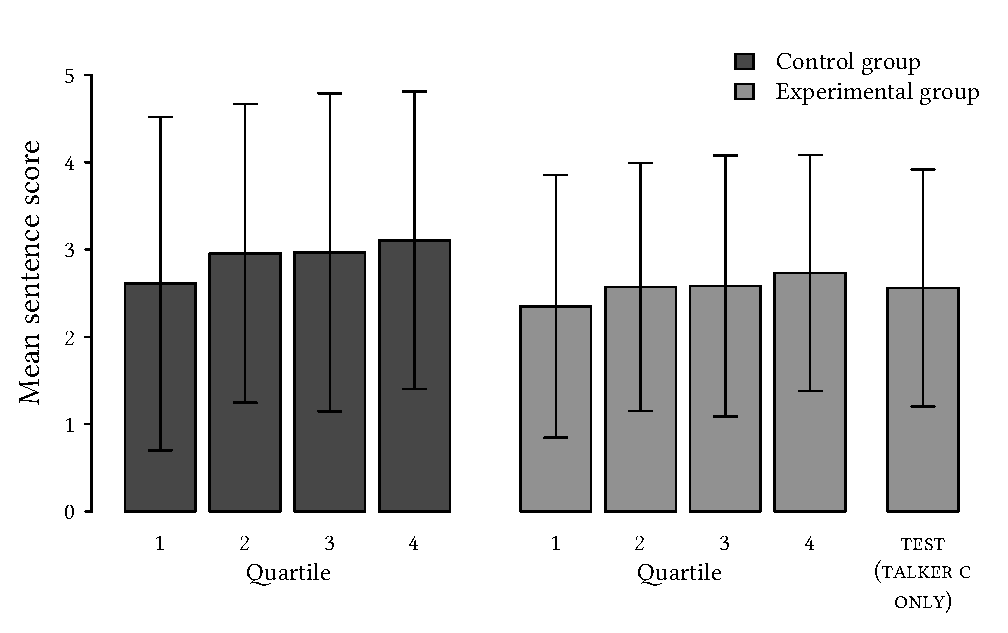
\includegraphics{figures/results/QuartileBarplot.eps}
	\caption[Quartile analysis of Experiment~2 training phase by group]{Quartile analysis of training phase in Experiment~2.  Improvement is seen during training for both the control group (trained on Talker~\ac{d}) and the experimental group (trained on Talker~\ac{c}).  The adaptation in the experimental group appears not to have persisted through the testing phase.\label{fig:Quartile}}
	\end{centering}
\end{figure}

For the experimental group, it appears that familiarization with Talker~\ac{c} during training did not confer an advantage on Talker~\ac{c} during testing (compare the last quartile of the training phase to the score on Talker~\ac{c} during the testing phase in Figure~\ref{fig:Quartile}).  %\footnotemark{}
%\footnotetext{This is true at least for the listeners trained on Talker~\ac{c}.  Listeners trained on Talker~\ac{d} did not hear their training talker during the testing phase, so it is unknown whether any adaptation was retained during testing.  Presumably, however, any such adaptation would have had little effect on performance when listening to Talkers~\ac{a}, \ac{b}, or \ac{c}.}
In light of this, it is perhaps unsurprising that training did not confer a reliable perceptual advantage on test stimuli resynthesized to have the training talker’s prosody; this is seen in the barplot of mean sentence scores for the testing phase of Experiment~2 (Figure~\ref{fig:ExpTwoBarplot}).  Even without controlling for multiple comparisons, none of the \textit{t}\=/tests comparing the experimental and control groups within talker are significant, suggesting that there was no familiar talker advantage enjoyed by the experimental group.  If there had been a familiar talker advantage, we would have expected the colored bars to be higher than their corresponding gray bars for Talker~\ac{c}, and perhaps for Talkers~\ac{ca}, \ac{cb}, \ac{ac} and \ac{bc} (depending on whether and how the advantage extended to resynthesized talkers).

\begin{figure}[bt]
	\begin{centering}
	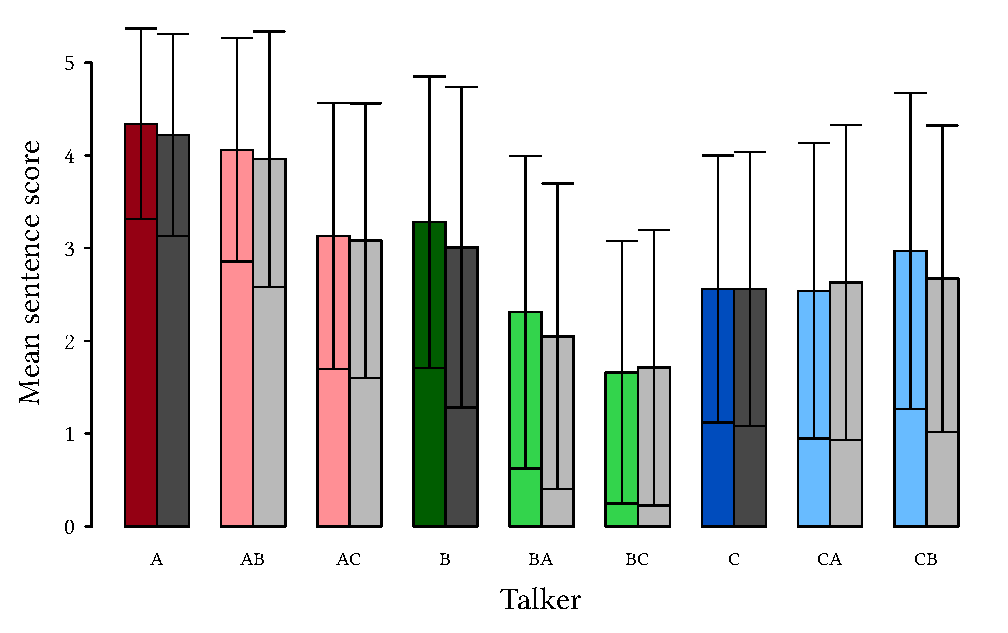
\includegraphics{figures/results/ExpTwoBarplot.eps}
	\caption[Barplot of mean sentence scores for Experiment~2]{Barplot of mean sentence scores for Experiment~2.  Error bars are ±1 standard error.  Colored bars indicate the experimental group; grayscale bars the control group.  Lighter colors indicate resynthesized talkers, and similar hues indicate shared segmental donors.\label{fig:ExpTwoBarplot}}
	\end{centering}
\end{figure}

\subsection{Experiment~2 statistical model}
Full results of the statistical model for Experiment~2 are shown in Table~\ref{tab:ExpTwoFixedEff}.  Predictor codes are the same as in the model for Experiment~1, with the addition of Boolean variables {\inlinecode segTrain} (indicating match between the training talker and the segmental donor of the test stimulus) and {\inlinecode proTrain} (indicating match between the training talker and the prosodic donor of the test stimulus).  

\begin{table}[tbp]
	\caption[Experiment~2 statistical model: Fixed effects]{Summary of fixed effect predictors in the statistical model of Experiment~2.  \textit{s}: standard error of the coefficient estimate; \textit{t}: \textit{t}\=/value of coefficient estimate; \textit{p}: \textit{p}\=/value of coefficient estimate (calculated via \ac{mcmc}).\label{tab:ExpTwoFixedEff}}
	\centering
	\begin{tabu} spread 1em {Xrcrc}
		\toprule
		\multicolumn{5}{l}{Summary of fixed effects (N=1800; log-likelihood=−3103)}\\
		\rowfont\bfseries
		\multicolumn{1}{l}{Predictor} & \multicolumn{1}{c}{Coefficient} & \textit{s} & \multicolumn{1}{c}{\itshape t} & \textit{p}\\
		\midrule
		Intercept	         &  4.366 & (0.139) &  31.50 & <10⁻¹⁶\\
		resynth = \ac{true}  & −0.603 & (0.066) &  −9.15 & <10⁻¹⁶\\
		segDonor = \ac{b}    & −1.466 & (0.075) & −19.42 & <10⁻¹⁶\\
		segDonor = \ac{c}    & −1.159 & (0.098) & −11.80 & <10⁻¹⁶\\
		proDonor = \ac{b}    &  0.270 & (0.075) &   3.60 & <10⁻³\\
		proDonor = \ac{c}    & −0.584 & (0.098) &  −5.95 & <10⁻⁸\\
		segTrain = \ac{true} &  0.008 & (0.125) &   0.06 & 0.95\\
		proTrain = \ac{true} & −0.117 & (0.125) &  −0.94 & 0.35\\
		trial                & −0.001 & (0.001) &  −0.64 & 0.53\\
		\bottomrule
	\end{tabu}
\end{table}

Unlike the model for Experiment~1, there is no significant effect for {\inlinecode trial} (unsurprising given Figure~\ref{fig:ExpTwoOctileBarplot}), most likely because listeners had already undergone a training phase and were already familiarized to the task.  Neither of the two new predictors {\inlinecode segTrain} and {\inlinecode proTrain} were significant, suggesting that listeners were not realizing a familiarity advantage due to training.  Aside from the lack of effect for {\inlinecode trial} and the two additional non\=/significant predictors {\inlinecode segTrain} and {\inlinecode proTrain}, the model is nearly identical to the model for Experiment~1; the magnitude, direction, and significance of the other fixed\-/effect predictors are all unchanged from Experiment~1.

A summary of the random effects in the model of Experiment~2 are shown in Table~\ref{tab:ExpTwoRandomEff}.  The results are also very similar to Experiment~1, with estimates of listener accounting for about 4\% of the total unexplained variability (with a standard deviation of 0.3 keywords) and sentence accounting for about 24\% of total unexplained variability (with a standard deviation of about 0.7 keywords).\footnotemark{}

\footnotetext{Again, \ac{mcmc} estimates for the effect of sentence were slightly smaller than the fitted model (18\% \vs\ 24\%), and there was close agreement between the two for the effect of listener.}

\begin{table}[tbp]
	\caption[Experiment~2 statistical model: Random effects]{Summary of random effects in the statistical model of Experiment~2.  \textit{s}²: estimated variance; \textit{s}: standard error; \ac{hpd}: highest posterior density interval.\label{tab:ExpTwoRandomEff}}
	\centering
	\begin{tabu} spread 1em {Xcccc}
		\toprule
		\multicolumn{3}{l}{Summary of random effects} & \multicolumn{2}{c}{\bfseries \ac{mcmc} (nsim=10\thinspace000)}\\ 
		\cmidrule{4-5}
		\rowfont\bfseries
		Group & \textit{s}² & \textit{s} & mean & 95\% \ac{hpd}\\
		\midrule
		Sentence (intercept) & 0.537 & 0.733 & 0.617 & (0.526~~0.712)\\
		Listener (intercept) & 0.083 & 0.288 & 0.297 & (0.192~~0.425)\\
		Residual             & 1.617 & 1.271 & 1.285 & (1.242~~1.329)\\
		\bottomrule
	\end{tabu}
\end{table}

\section{\Ph{} acoustic analyses}
Overall, the statistical models for Experiments~1 and~2 support the view that both prosodic and non\=/prosodic factors contribute to differences in the intelligibility of talkers.  To better understand these results, a variety of acoustic measurements were performed on the stimuli, in hopes of identifying the acoustic dimensions that underlie the effects seen in the statistical models.  The measures are broadly divided into segmental measures (presence of stop release bursts, properties of the vowel space) and prosodic measures (mean pitch range, pitch velocity, pitch dynamicity, intensity velocity, intensity dynamicity, and syllable duration).

\subsection{Segmental measures}
The results of the stop consonant reduction analysis are shown in Figure~\ref{fig:ReleaseBursts}.  The percentages given are calculated as the total number of stops and affricates counted (across the 45 sentences measured) divided by the total number of expected stop consonants based on citation\-/form phonemic transcriptions; there was little difference between this method and the method of calculating the mean of unreduced stop percentage calculated on a per-stimulus basis.  The relative ordering of the talkers accords with their relative intelligibility (\ie, Talker~\ac{a}~> Talker~\ac{b}~> Talker~\ac{c}), but does not correspond to the expected ordering based on coefficients for segmental donor (\ac{a}~> \ac{c}~> \ac{b}).  

\begin{figure}[bt]
	\begin{centering}
	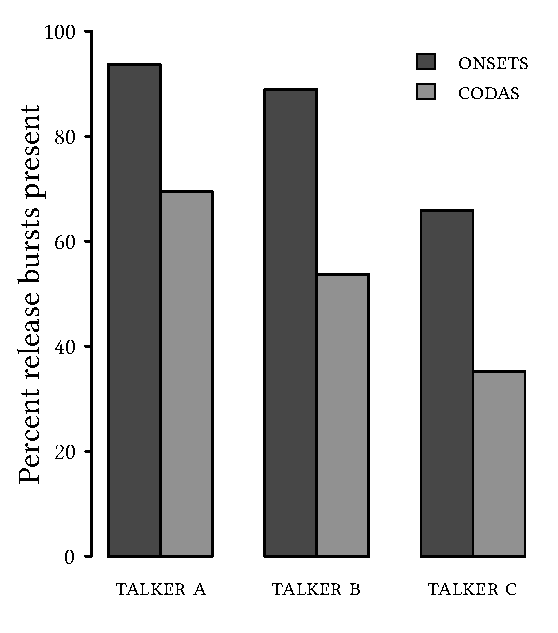
\includegraphics{figures/posthocs/ReleaseBursts.eps}
	\caption[Barplot of mean proportion of unreduced stop consonants]{Barplot of mean proportion of unreduced stop consonants present, calculated across half of the test stimuli (45 sentences per talker).\label{fig:ReleaseBursts}}
	\end{centering}
\end{figure}

A possible explanation for the ordering of talkers is that stop reduction may index both segmental and prosodic information, for two reasons: first, stop consonants often occur at word edges, which are loci for word\-/level prosodic marking, and second, stop consonants are often strengthened in prosodically prominent syllables at higher levels of phrasal structure (cf., \eg, \citealt{deJong1995, FougeronKeating1997, ChoEtAl2007, ColeEtAl2007}; see \citealt{Keating2006} for review).  In other words, because stop consonant reduction was measured across all words in the sentence, it may reflect a combination of each talker’s prosodic habits (\ie, tendency toward more \vs\ fewer intonational phrases) as well as purely segmental pronunciation habits (which might have been more easily observed from words lists).  Unfortunately, the \ac{pn/nc} corpus does not include recordings of word lists, so this explanation must remain speculative.

Results of the \ph{} analysis of vowel space size is shown in Figure~\ref{fig:VowelSpace}.  Here the expected pattern of \ac{a}~> \ac{c}~> \ac{b} (based on coefficients for segmental donor from Experiments~1 and~2) is seen in three of the five measures: mean distance from center, area of the convex hull, and F1 range.  F2 range does not correlate with any expected intelligibility-related pattern, while area of the polygon based on vowel means seems to correlate with overall intelligibility scores for each talker (\ie, \ac{a}~> \ac{b}~> \ac{c}).  

\begin{figure}[bt]
	\begin{centering}
	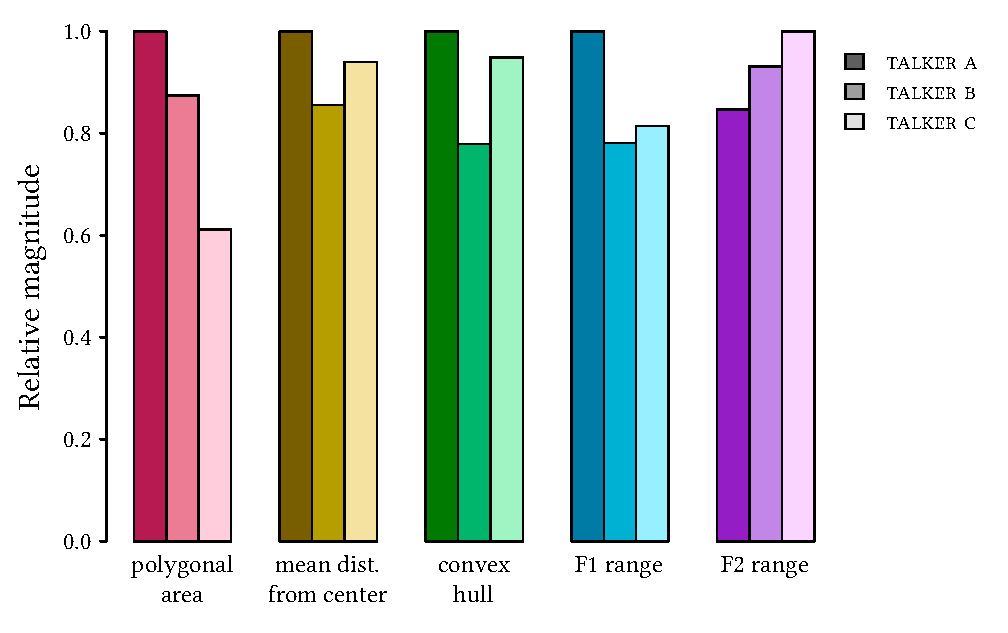
\includegraphics{figures/posthocs/VowelSpace.eps}
	\caption[Barplot of vowel space size metrics]{Barplot of the relative magnitudes of several vowel space size metrics.  Each metric has been scaled by dividing by the maximum value among the three talkers.\label{fig:VowelSpace}}
	\end{centering}
\end{figure}

The difference between area of the convex hull and area of the vowel means polygon is especially interesting.  Figure~\ref{fig:ConvexHull} plots both the convex hull and vowel means polygons on data from Talker~\ac{a}.  This figure illustrates one possible explanation for the difference in patterning between these two measures of vowel space size: the convex hull effectively ignores vowel tokens that are reduced (for any reason) — and thus indexes a talker’s most extreme vowel productions — whereas the area of the vowel means polygon includes information from multiple vowel tokens, which may show reduction due to prosodic differences between talkers (because the tokens came from various positions within the sentence).  Considering that all the vowel tokens measured came from lexically stressed syllables in content words, any vowel quality reduction present in these tokens is \emph{not} reduction due to lack of \emph{lexical} stress; thus it is quite likely that the reduction seen is prosodic in origin.

\begin{figure}[bt]
	\begin{centering}
	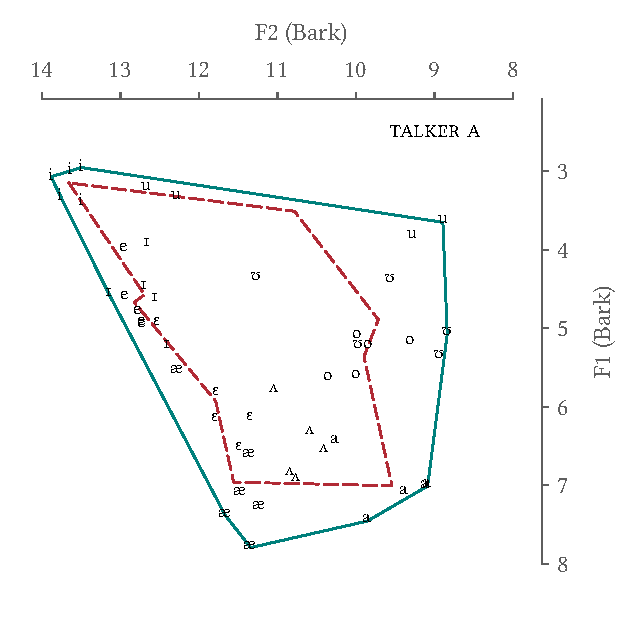
\includegraphics{figures/posthocs/ConvexHull.eps}
	\caption[Vowel space metrics]{Illustration of two vowel space area metrics (data from Talker~\ac{a}).  The area of the polygon described by vowel means (dashed red line) is contrasted with the convex polygonal hull (solid blue line).  Note the difference between the polygons in the high\-/back and low\-/front regions due to /u/-fronting and /æ/-raising (respectively), as well as differences due to reduction (particularly in the /o/, /ʊ/ and /ɛ/ regions).\label{fig:ConvexHull}}
	\end{centering}
\end{figure}

The distribution of vowel tokens in Figure~\ref{fig:ConvexHull} also shows some within\-/category variation that is probably not due to prosodically\-/driven reduction.  For example, the large variation in F2 of the high back vowel /u/ is likely an example of the widespread change\-/in\-/progress known as /u/-fronting \citep[chap.\ 12]{LabovEtAl2006}.  Similar variation is seen in F1 values for /æ/ (cf. reports of /æ/-raising before velars in the Pacific Northwest: \citealt{Reed1952, WassinkEtAl2009}).  Such cases also affect measures of vowel means polygonal area, but are less likely to impact measures of convex hull area (as seen in the high\-/back and low\-/front regions of Figure~\ref{fig:ConvexHull}).  In this way, area of the vowel means polygon could be said to contain information about both segmental and prosodic dimensions of speech (much like stop consonant reduction discussed above), which may explain why it corresponds to the ordering of talkers based on general intelligibility scores, rather than the ordering of talkers based on segmental donor coefficients in the statistical models.  In contrast, area of the convex hull may be a better index of purely segmental properties of speech, since it ignores within-category variation of vowels (at least some of which is prosodically\-/driven); this would explain why area of the convex hull correlates with the ordering of talkers based on signal donor coefficients.\footnotemark{}

\footnotetext{Note that although area of the convex hull appears to be less sensitive than the area of the vowel means polygon to phonological variation such as /u/-fronting and /æ/-raising, it is not completely immune to such influence.  As such, care should be used when comparing across dialects or sociolects where the presence or degree of such features is not consistent across groups.}

The preceding discussion suggests that a thorough analysis of the vowel space would segregate measures of overall vowel space expansion from measures of individual vowel category size, and would include some measure of category overlap or encroachment.  To explore this need, measures of mean cluster size and repulsive force of each talker’s vowel system are shown in Figure~\ref{fig:ForceCluster} (see Section~\ref{sec:SegmentalMethods} for definition of these measures).

\begin{figure}[bt]
	\begin{centering}
	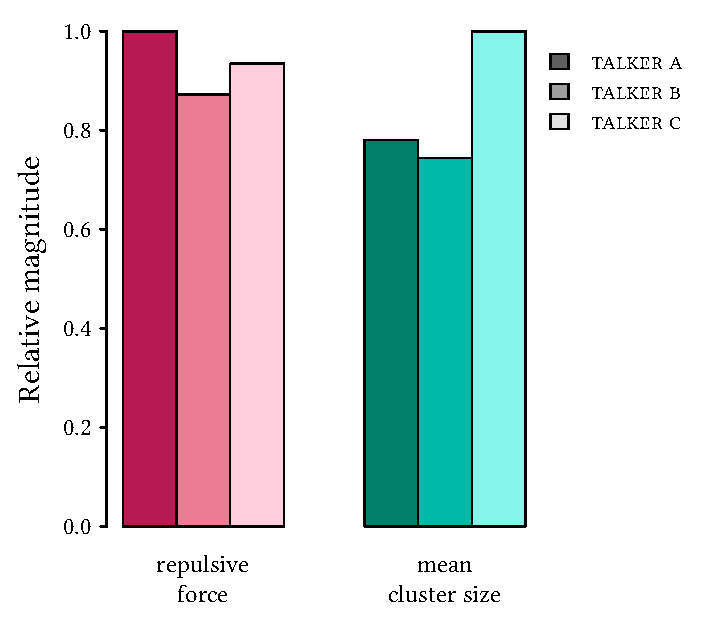
\includegraphics{figures/posthocs/ForceCluster.eps}
	\caption[Barplot of vowel overlap and encroachment metrics]{Barplot of the relative magnitudes of mean vowel cluster size and repulsive force.  Each metric has been scaled by dividing by the maximum value among the three talkers.\label{fig:ForceCluster}}
	\end{centering}
\end{figure}

A high degree of repulsive force indexes a high degree of phonemic overlap, which ought to correspond to \emph{lower} intelligibility (on the assumption that words would be more confusable in talkers whose phonemic categories are not well segregated).  Thus the expected pattern based on the statistical model coefficients for segmental donor ought to be \ac{b}~> \ac{c}~> \ac{a}, which is precisely the opposite of the pattern seen in Figure~\ref{fig:ForceCluster}.  It is possible that fifty vowel tokens (five per vowel) was simply not a large enough number to give an accurate picture of the internal structure of the vowel space.  In any case, the likelihood of lexical confusion due to vowel phoneme overlap is contingent on the existence and lexical probability of the competing form.  For example, no matter how much /u/-fronting a talker exhibits, the /u/ vowel in “poodles” (sentence 15–06) is unlikely to be heard as /i/.  Duration is also relevant: although “kits” and “Kate’s” are potentially confusable based on formant values (see Talker~\ac{a}’s vowel plot in Figure~\ref{fig:ConvexHull}), there are likely to be duration differences that listeners can rely on to disambiguate the two forms.  Thus it is perhaps unsurprising that repulsive force is a poor predictor in a sentence perception task such as this one (as opposed to an isolated word perception task in which stimuli are chosen to ensure the viability of competing forms, and plausibility is not constrained by semantic context).

Mean cluster size should index within\-/category variability of vowel formants, and is predicted (like repulsive force) to be inversely correlated with the non\-/prosodic component of intelligibility.  However, like repulsive force, the magnitudes of mean cluster size also fail to track the expected pattern of \ac{b}~> \ac{c}~> \ac{a}.  Again, a possible explanation is that an insufficient number of vowel tokens were available to give accurate estimates of the spectral extent of within\-/category variation.  Another explanation is that because mean cluster size collapses information across vowels, it does not distinguish differences in crowded parts of the vowel space (likely to cause confusions) from differences in sparse regions (unlikely to cause confusions).  This suggests the need for a hybrid measure somehow encompassing both within\-/category variation and category overlap or encroachment.  More research is needed to determine how such a measure could be derived.

\subsection{Prosodic measures}
\begin{figure}[bt]
	\begin{centering}
	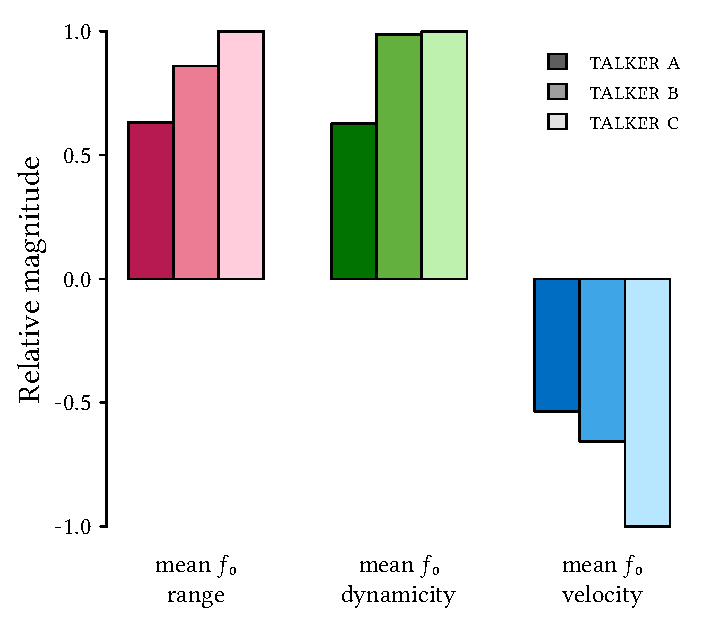
\includegraphics{figures/posthocs/ProsodicMeasuresPitchOnly.eps}
	\caption[Barplot of \fo{} metrics]{Barplot of the relative magnitudes of three \fo-related metrics.  Each metric has been scaled by dividing by the maximum absolute value among the three talkers.\label{fig:ProsodicMeasuresPitch}}
	\end{centering}
\end{figure}

\Ph{} analyses of the prosodic measures related to \fo{} are shown in Figure~\ref{fig:ProsodicMeasuresPitch}.  The expected pattern based on statistical model coefficients for prosodic donor is Talker~\ac{b}~> Talker~\ac{a}~> Talker~\ac{c}.  None of the three measures match this pattern exactly; the closest is mean \fo{} dynamicity, which shows a pattern of \ac{b}~≈ \ac{c}~> \ac{a}.  Mean \fo{} range shows a pattern of \ac{c}~> \ac{b}~> \ac{a}, as does mean \fo{} velocity (in the case of velocity, “>” meaning “more negative”).\footnotemark{}  One explanation that ties these three measures together is the fact that Talker~\ac{c} exhibits a lot of creaky voicing in his speech, especially utterance\-/finally, which accounts for his highly negative value of \fo{} velocity (nearly twice the magnitude of Talker~\ac{a}).  The relatively frequent occurrence of creaky voicing in Talker~\ac{c}’s stimulus sentences can be seen in Figure~\ref{fig:PitchTracks}, by the high number of “tails” protruding downward from the main mass of pitch tracks at the ends of several sentences.
\footnotetext{Recall that dynamicity is a measure of the mean of the \emph{absolute value} in rate of change of \fo, whereas velocity is the mean of the signed rate of change.  As such, velocity reflects overall trends in pitch across the utterance, whereas dynamicity better indexes the magnitude of pitch movements throughout the utterance.}

\begin{figure}[pbt]
	\begin{centering}
	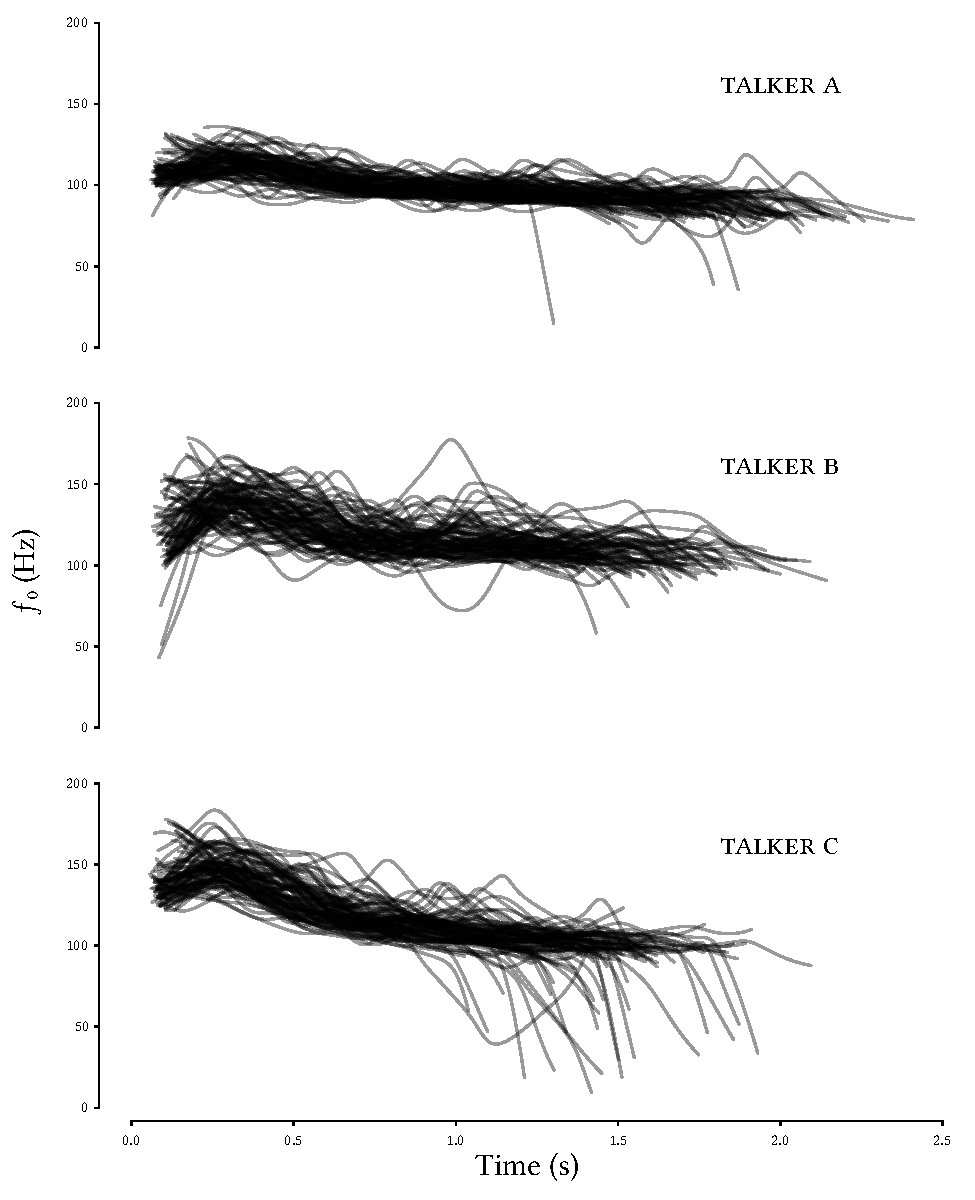
\includegraphics{figures/posthocs/PitchTracks.pdf}
	\caption[Pitch track overlays of the test sentences]{Overlaid pitch tracks for Talkers~\ac{a}, \ac{b} and~\ac{c} for the 90 test sentences.  Pitch tracks have been smoothed by fitting a local polynomial weighted by a Gaussian kernel with a bandwidth of 75 ms.  Note the frequent occurrence of utterance\-/final creaky voicing (indicated by extreme drops in \fo) for Talker~\ac{c}.\label{fig:PitchTracks}}
	\end{centering}
\end{figure}

The consistent use of creaky voicing also inflates Talker~\ac{c}’s values for mean \fo{} range and mean \fo{} dynamicity.  Re\=/examining Figure~\ref{fig:ProsodicMeasuresPitch} in this light, we see that both mean \fo{} range and mean \fo{} dynamicity show the expected relationship between Talkers~\ac{a} and~\ac{b}.  Figure~\ref{fig:PitchTracks} also visually illustrates Talker~\ac{a}’s low \fo{} range (the tighter clustering of his pitch tracks compared to Talker~\ac{b}) and dynamicity (the straightness of the lines in his pitch tracks compared to Talker~\ac{b}).

\begin{figure}[bt]
	\begin{centering}
	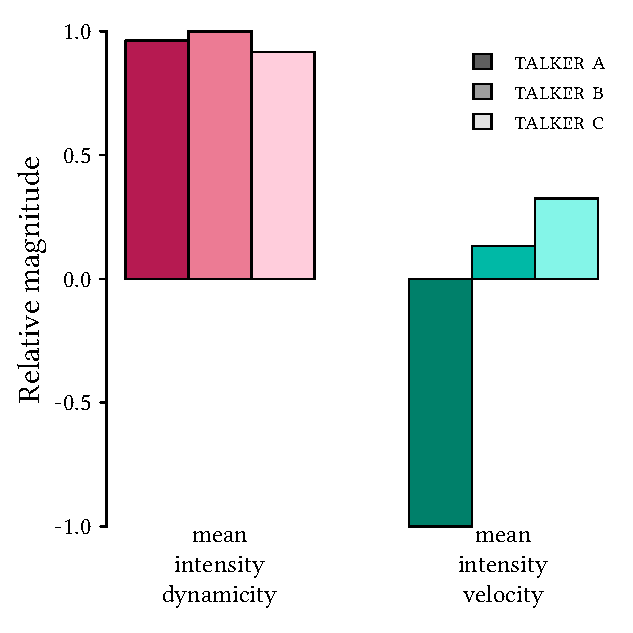
\includegraphics{figures/posthocs/ProsodicMeasuresIntensityOnly.eps}
	\caption[Barplot of intensity metrics]{Barplot of the relative magnitudes of two intensity-related metrics.  Each metric has been scaled by dividing by the maximum absolute value among the three talkers.\label{fig:ProsodicMeasuresIntensity}}
	\end{centering}
\end{figure}

\Ph{} analyses of the prosodic measures related to intensity are seen in Figure~\ref{fig:ProsodicMeasuresIntensity}.  The values for mean intensity dynamicity follow the predicted pattern of \ac{b}~> \ac{a}~> \ac{c}, but only the difference between Talkers~\ac{b} and~\ac{c} is significant.  The small differences between talkers is probably due to the fact that intensity dynamicity mostly tracks something like obstruent\slsh sonorant alternation rate, since the largest\-/magnitude intensity modulations in speech (at all but the shortest time scales) are the inherent differences between segment types — voiceless stop closures at one extreme, and open vowels at the other (cf. the well\-/known linguistic notion of \term{sonority}).  Because all talkers read the same set of sentences, the patterns of obstruent\-/sonorant alternation were by and large identical across talkers (modulo variation due to segmental reduction) and therefore any variation due to inter\-/talker differences in prosody are likely to be relatively small in comparison (and thus hard to detect statistically).

\begin{figure}[pbt]
	\begin{centering}
	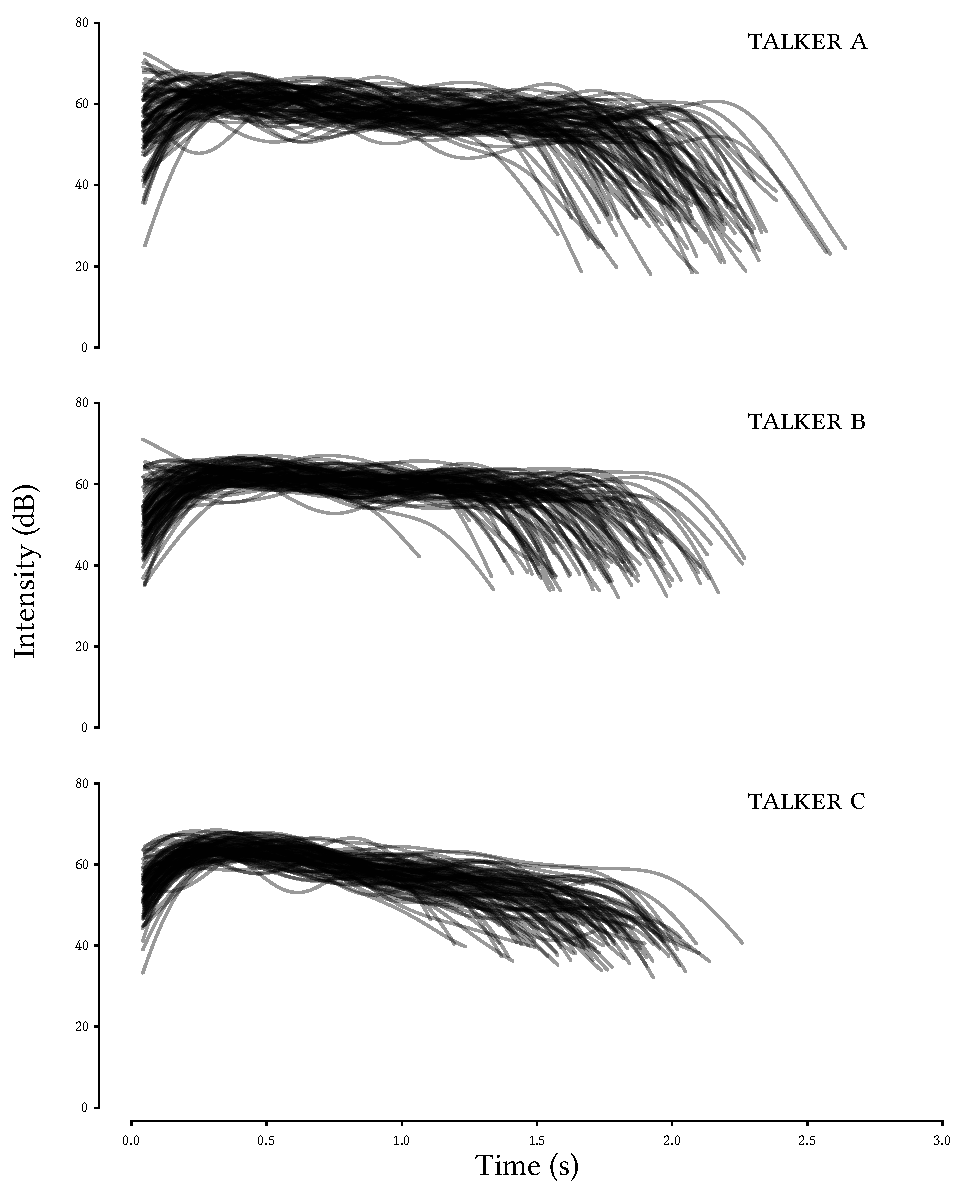
\includegraphics{figures/posthocs/IntensityTracks.pdf}
	\caption[Intensity track overlays of the test sentences]{Overlaid pitch tracks for Talkers~\ac{a}, \ac{b} and~\ac{c} for the 90 test sentences.  Pitch tracks have been heavily smoothed by fitting a local polynomial weighted by a Gaussian kernel with a bandwidth of 150 ms.\label{fig:IntensityTracks}}
	\end{centering}
\end{figure}

Values for mean intensity velocity show an unusual pattern in which Talker~\ac{a} shows an extreme negative value, with Talkers~\ac{b} and~\ac{c} showing small positive values (see Figure~\ref{fig:ProsodicMeasuresIntensity}).  Some insight into this pattern is available if we examine the overlaid intensity tracks for each talker, as seen in Figure~\ref{fig:IntensityTracks}.  At the expense of showing detail at smaller time scales, the wide (150~ms) smoothing bandwidth highlights the overall trends in intensity in each recording, and reveals the strong intensity drop\=/off at the end of most of Talker~\ac{a}’s sentences, the smaller drop\=/off in Talker~\ac{b}’s speech, and the tendency for Talker~\ac{c}’s speech to decline more gradually in intensity across the sentence.  The strong drop\=/off is responsible for Talker~\ac{a}’s large negative value for mean intensity velocity seen in Figure~\ref{fig:ProsodicMeasuresIntensity}; in fact, given that mean intensity velocity is anticorrelated with talker intelligibility, we can infer that the strong drop\=/off is probably less damaging to the intelligibility of speech in noise than a gradual decline.  This makes sense if Talker~\ac{a}’s tendency for utterance\-/final drop\=/off likely only affects the last word, whereas Talker~\ac{c}’s tendency for more gradual intensity decline gradually reduces \ac{snr} for words occurring mid\=/sentence.

\begin{figure}[bt]
	\begin{centering}
	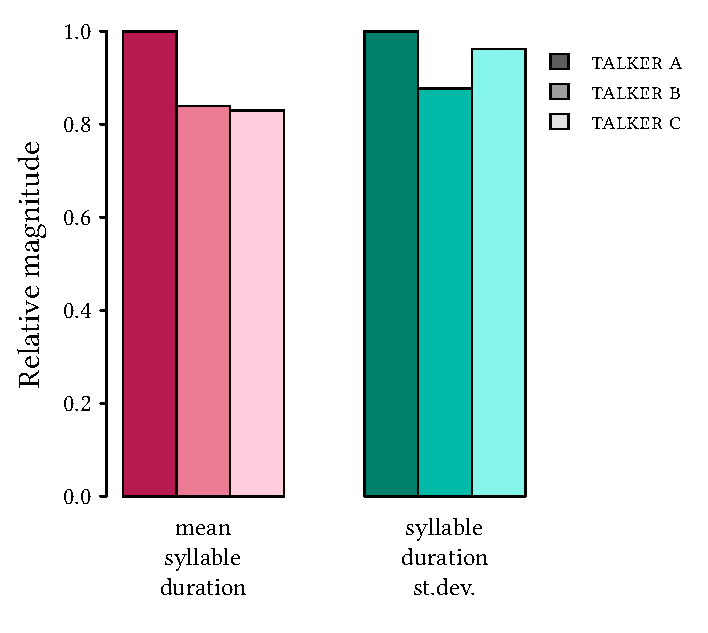
\includegraphics{figures/posthocs/SyllableDuration.eps}
	\caption[Barplot of duration metrics]{Barplot of the relative magnitudes of two duration-related metrics.  Each metric has been scaled by dividing by the maximum absolute value among the three talkers.\label{fig:SyllableDuration}}
	\end{centering}
\end{figure}

\Ph{} analyses of syllable duration are seen in Figure~\ref{fig:SyllableDuration}.  Mean syllable duration for Talkers~\ac{b} and~\ac{c} is nearly identical, and thus cannot explain the difference in intelligibility between them.  This is consistent with findings in the literature suggesting that within\-/talker changes in intelligibility are not necessarily accompanied by a change in speech rate \citep{KrauseBraida2002}; further interpretation of mean speech rate values is limited by the small number of talkers investigated here.  Interestingly, \emph{variability} in syllable duration appears to follow the pattern of non\=/prosodic coefficients (\ie, \ac{a}~> \ac{c}~> \ac{b}).  This is unexpected, since large variability in syllable duration is expected to index more extreme duration contrasts between prominent and reduced syllables (more a prosodic phenomenon than a segmental or lexical one).  This result also merits further investigation with a larger sample of talkers.

% \subsection{\Ph{} statistical analysis}
